\begin{figure}[htbp]
    \centering
    % Load required TikZ libraries
    \usetikzlibrary{backgrounds,fit,calc,shapes.geometric,shadows,arrows.meta,positioning,shapes.multipart}
    \pgfdeclarelayer{background}
    \pgfsetlayers{background,main}
    \resizebox{\linewidth}{!}{
    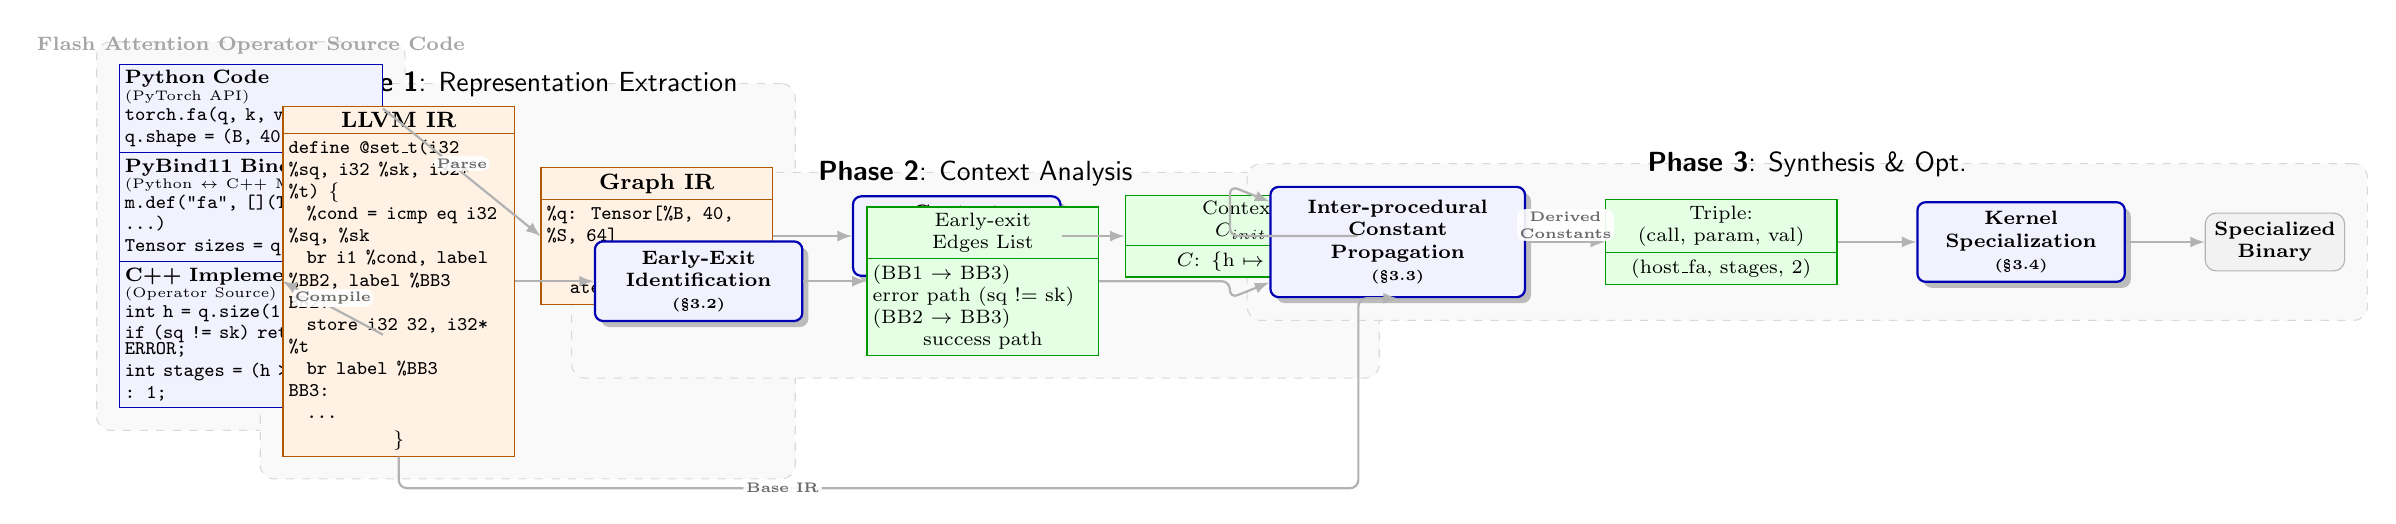
\begin{tikzpicture}[
        % 全局样式设置
        font=\sffamily,
        node distance=1.0cm and 1.5cm,
        >=latex,
        % --- 节点样式 ---
        % 蓝色算子/处理模块
        process/.style={
            rectangle,
            draw=blue!70!black,
            fill=blue!5,
            rounded corners=3pt,
            minimum height=1.0cm,
            text width=2.4cm,
            align=center,
            thick,
            font=\scriptsize\bfseries,
            drop shadow
        },
        % 橙色 IR 表示
        ir/.style={
            trapezium,
            trapezium left angle=70,
            trapezium right angle=110,
            draw=orange!70!black,
            fill=orange!10,
            minimum height=0.8cm,
            text width=1.8cm,
            align=center,
            font=\footnotesize\bfseries
        },
        % 橙色 IR 文本框 (带代码示例)
        irbox/.style={
            rectangle split,
            rectangle split parts=2,
            draw=orange!70!black,
            fill=orange!10,
            rectangle split part fill={orange!20, orange!5},
            minimum height=1.5cm,
            text width=2.8cm,
            align=center,
            font=\footnotesize\bfseries,
            inner sep=2pt
        },
        % 绿色 数据/中间结果
        data/.style={
            trapezium,
            trapezium left angle=110,
            trapezium right angle=70,
            draw=green!60!black,
            fill=green!10,
            minimum height=0.7cm,
            text width=1.6cm,
            align=center,
            font=\scriptsize
        },
        % 绿色 数据文本框 (带代码示例)
        databox/.style={
            rectangle split,
            rectangle split parts=2,
            draw=green!60!black,
            fill=green!10,
            rectangle split part fill={green!20, green!5},
            minimum height=1.5cm,
            text width=2.8cm,
            align=center,
            font=\scriptsize,
            inner sep=2pt
        },
        % 源码层级框
        sourcebox/.style={
            rectangle,
            draw=gray!40,
            fill=gray!2,
            rounded corners=2pt,
            text width=3.2cm,
            align=center,
            font=\scriptsize,
            inner sep=3pt
        },
        % 源码文本框 (带标题和代码)
        sourcebox2/.style={
            rectangle split,
            rectangle split parts=2,
            draw=blue!70!black,
            fill=blue!5,
            rectangle split part fill={blue!20, blue!5},
            minimum height=1.5cm,
            text width=3.2cm,
            align=center,
            font=\scriptsize,
            inner sep=2pt
        },
        % 源码单框 (三个部分)
        sourcebox3/.style={
            rectangle split,
            rectangle split parts=3,
            draw=blue!70!black,
            fill=blue!5,
            rectangle split part fill={blue!20, gray!20, orange!20},
            minimum height=3.5cm,
            text width=3.2cm,
            align=left,
            font=\scriptsize,
            inner sep=2pt
        },
        % 背景分区框
        groupbox/.style={
            rectangle,
            draw=gray!30,
            fill=gray!5,
            dashed,
            rounded corners=5pt,
            inner sep=8pt
        },
        % 标签文字
        labeltext/.style={
            font=\tiny\bfseries, 
            color=gray!70!black, 
            align=center,
            fill=white, 
            inner sep=1pt,
            opacity=0.9
        },
        % 连线
        arrow/.style={->, thick, draw=gray!60, rounded corners=3pt},
        % 代码示例样式
        codebox/.style={
            rectangle,
            draw=none,
            fill=none,
            font=\ttfamily\tiny,
            align=left,
            inner sep=1pt,
            text width=2.8cm
        }
    ]

    % ============================================================
    % 1. 左侧：Flash Attention Operator Source Code (源码层)
    % ============================================================
    % Flash Attention Operator Source Code (single box with three parts)
    \node (py_layer) [sourcebox3, text width=3.2cm] {
        \textbf{Python Code}\\
        \tiny (PyTorch API)\\
        {\ttfamily\scriptsize torch.fa(q, k, v, lens)}\\
        {\ttfamily\scriptsize q.shape = (B, 40, S, 64)}
        \nodepart{second}
        \textbf{PyBind11 Binding}\\
        \tiny (Python $\leftrightarrow$ C++ Map)\\
        {\ttfamily\scriptsize m.def("fa", [](Tensor q, ...)}\\
        {\ttfamily\scriptsize Tensor sizes = q.sizes();}
        \nodepart{third}
        \textbf{C++ Implementation}\\
        \tiny (Operator Source)\\
        {\ttfamily\scriptsize int h = q.size(1); // 40}\\
        {\ttfamily\scriptsize if (sq != sk) return ERROR;}\\
        {\ttfamily\scriptsize int stages = (h > 32) ? 2 : 1;}
    };
    
    % 源码组标题
    \node [above=0pt of py_layer, font=\bfseries\scriptsize, color=gray!70] {Flash Attention Operator Source Code};

    % 背景框：Flash Attention Operator Source Code
    \begin{pgfonlayer}{background}
        \node [groupbox, fit=(py_layer)] (sourcegroup) {};
    \end{pgfonlayer}

    % ============================================================
    % 2. 中间分层：Dynamic (上) vs Static (下)
    % ============================================================
    
    % --- 上层流：Dynamic / Graph IR ---
    % Graph IR 与 Python 层对齐
    \node (graphir) [irbox, right=2.0cm of py_layer] {Graph IR \nodepart{second} \raggedright{\ttfamily\scriptsize \%q: Tensor[\%B, 40, \%S, 64]\\ \%out = aten::fa(\%q, ...)}};
    \node (ctxgen) [process, right=1.0cm of graphir] {Context\\Generation\\\tiny(\S3.1)};
    \node (context) [databox, right=0.8cm of ctxgen] {Context\\$\mathbb{C}_{init}$ \nodepart{second} \raggedright$\mathbb{C}$: \{h $\mapsto$ 40\}};
    
    % --- 下层流：Static / LLVM IR ---
    % LLVM IR 与 C++ 层对齐
    \node (llvmir) [irbox, right=2.0cm of py_layer.three] {LLVM IR \nodepart{second} \raggedright{\ttfamily\scriptsize define @set\_t(i32 \%sq, i32 \%sk, i32* \%t) \{\\\ \ \%cond = icmp eq i32 \%sq, \%sk\\\ \ br i1 \%cond, label \%BB2, label \%BB3\\BB2:\\\ \ store i32 32, i32* \%t\\\ \ br label \%BB3\\BB3:\\\ \ ...\\\}}};
    \node (earlyexit) [process, right=1.0cm of llvmir] {Early-Exit\\Identification\\\tiny(\S3.2)};
    \node (edges) [databox, right=0.8cm of earlyexit] {Early-exit\\Edges List \nodepart{second} \raggedright (BB1 $\rightarrow$ BB3)\\ error path (sq != sk)\\ (BB2 $\rightarrow$ BB3)\\ success path};

    % ============================================================
    % 3. 右侧：核心汇聚与特化
    % ============================================================
    
    % Constant Propagation 位于 Context 和 Edges 的垂直中间
    % 利用 calc 库计算中间位置
    \coordinate (midpoint) at ($(context.south)!0.5!(edges.north)$);
    
    % 核心模块：Constant Propagation
    \node (constprop) [process, right=2.0cm of midpoint, anchor=west, minimum height=1.4cm, text width=3cm] {
        Inter-procedural\\Constant Propagation\\\tiny(\S3.3)
    };
    
    % Kernel Specialization
    \node (triples) [databox, right=1.0cm of constprop] {Triple:\\(call, param, val) \nodepart{second} \raggedright (host\_fa, stages, 2)};
    \node (kernelspec) [process, right=1.0cm of triples] {Kernel\\Specialization\\\tiny(\S3.4)};
    
    % Final Output
    \node (final) [rectangle, draw=gray!60, fill=gray!10, right=1.0cm of kernelspec, font=\scriptsize\bfseries, align=center, rounded corners] {Specialized\\Binary};

    % ============================================================
    % 4. 连线 (Arrows)
    % ============================================================
    
    % 左侧映射
    \draw[arrow] (py_layer.one east) -- node[above, labeltext] {Parse} (graphir.west);
    \draw[arrow] (py_layer.three east) -- node[above, labeltext] {Compile} (llvmir.west);
    
    % 上层流 (Dynamic)
    \draw[arrow] (graphir) -- (ctxgen);
    \draw[arrow] (ctxgen) -- (context);
    
    % 下层流 (Static)
    \draw[arrow] (llvmir) -- (earlyexit);
    \draw[arrow] (earlyexit) -- (edges);
    
    % *** 关键汇聚逻辑 ***
    % 1. Context (Dynamic Info) -> ConstProp
    \draw[arrow] (context.east) -| ([xshift=-0.5cm]constprop.north west) -- ([yshift=-0.2cm]constprop.north west);
    
    % 2. Edges (Pruning Info) -> ConstProp
    \draw[arrow] (edges.east) -| ([xshift=-0.5cm]constprop.south west) -- ([yshift=0.2cm]constprop.south west);
    
    % 3. LLVM IR (Static Graph) -> ConstProp
    % 这条线最长，需要穿过中间。表示 ConstProp 是在 LLVM IR 上运行的
    \draw[arrow] (llvmir.south) -- ++(0,-0.4) -| node[pos=0.2, labeltext] {Base IR} ([xshift=-0.5cm]constprop.south) -- (constprop.south);
    
    % 后续流
    \draw[arrow] (constprop) -- node[above, labeltext] {Derived\\Constants} (triples);
    \draw[arrow] (triples) -- (kernelspec);
    \draw[arrow] (kernelspec) -- (final);

    % ============================================================
    % 5. 背景分区 (Background Layers)
    % ============================================================
    \begin{pgfonlayer}{background}
        % Phase 1: IR Extraction
        \node [groupbox, fit=(graphir) (llvmir), label={[shift={(0,-2ex)}]north:\textbf{Phase 1}: Representation Extraction}] (phase1) {};
        
        % Phase 2: Analysis
        \node [groupbox, fit=(ctxgen) (earlyexit) (context) (edges), label={[shift={(0,-2ex)}]north:\textbf{Phase 2}: Context Analysis}] (phase2) {};
        
        % Phase 3: Optimization
        \node [groupbox, fit=(constprop) (kernelspec) (final), label={[shift={(0,-2ex)}]north:\textbf{Phase 3}: Synthesis \& Opt.}] (phase3) {};
    \end{pgfonlayer}
    
    % ============================================================
    % 6. 示例标注 (Example Annotations)
    % ============================================================

    \end{tikzpicture}
    }
    \caption{Workflow of TilingInfer. The pipeline extracts dynamic context from Graph IR (top stream) and static structure from LLVM IR (bottom stream). These streams converge at the Constant Propagation engine (Phase 3) to generate specialized kernels. The diagram includes example code snippets from Flash Attention (Python DSL, PyBind, C++) and early‑exit edges from the sanity‑check example.}
    \label{fig:tilinginfer_workflow}
    \vspace{-10pt}
\end{figure}